\section{Analysis of Truthful Reporting in MAB with private payoff}
\label{app:analysis_mab}

\begin{proposition}[Truthful reporting is interim strictly dominant in one round]
  \label{prop:dominance}
  In one round, truthful reporting is a interim strictly dominant strategy for the sender \cref{eq:reward} if $p\,(\eta+\varphi) > \eta\,\sbar+\Gamma$ and $p\eta>\xi$.

\end{proposition}

\begin{proof}
  Let us reconsider the problem introduced in \cref{sec:problem}. We relax the problem into a single round with one sender. Thus, for brevity, we will drop the "$t$" notation. In this case, a \emph{sender} $i$ found an arm, and choose to make an report $m\in\{\varnothing\}\cup\mathbb R_{>0}$. A report $m$ is truthful if $m=\theta$ and untruthful otherwise, whether exaggerated ($m>\theta$) or understated ($m<\theta$), and $m=\varnothing$ is silence. Everyone else, receivers and other senders, is collapsed into an arbitrary \emph{opponent profile}, denoted $\sigma_{-i}$: any map from the posted claim to a distribution over their actions.

We assume the follows.

\begin{enumerate}[label=A\arabic*]
  \item \emph{Separability.} Given the action profile, $u_i$ does not depend on $m_i$. Claims affect $i$'s reward only through $C_i$ and through receivers' future behaviour.
  \item \emph{Unforgeable verification.} On checked claims the designer learns $\theta_i$ exactly, and followers cannot misreport it.
  \item \emph{Independent audits.} $a_i$ is independent of $(m, d, h)$.
  \item \emph{Untruthful reports are detected.} Every untruthful report, whether exaggerated or understated, misses the tolerance: $m\neq\theta \Rightarrow |m/\theta-1|>\tau$.
  \item \emph{Truthful reports do not hurt the sender.} A truthful report does not lower the sender's weighted payoff $(1-\lambda)u_i+\lambda\bar u_{-i}$ relative to silence. This holds when receivers never follow a truthful claim at a loss to themselves and following does not change the sender's own payoff.
\end{enumerate}

\begin{table}[t]
  \caption{Reward $r$ of a sender $i$ under \tvc{} in one round, based on \cref{eq:reward}, in units of $\vbar$. Each row is what happens to the claim: whether some receiver follows it and whether the random audit checks it. Each column is what the sender does: report truthfully ($m=\theta$), report untruthfully ($m\neq\theta$, exaggerated or understated) or stay silent ($m=\varnothing$). Each cell is \cref{eq:reward} evaluated with the credit of \cref{eq:tvc} for the case in its row and column, with $S=S(m,\theta)$. Every claim bears the posting cost $\xi$. An untruthful report never passes the verification gate, so it earns no gain credit, and it gains the outside gain $\Gamma$ only when it is followed, because only then do believers act on it. We take the outside effect of a truthful claim as zero, since a positive effect only favours truth. Silence posts no claim, so it bears no cost and earns $0$.}
  \label{tab:cases}
  \centering
  \small
  \setlength{\textwidth}{3pt}
  \begin{tabular}{lccc}
    \toprule
    Case & Truth & Untruthful & Silence \\
    \midrule
    Followed, audited         & $\min(g,\Bbar)+\eta-\xi$ & $\Gamma+\eta S-\varphi-\xi$ & $0$ \\
    Followed, not audited     & $\min(g,\Bbar)+\eta-\xi$ & $\Gamma+\eta S-\xi$         & $0$ \\
    Not followed, audited     & $\eta-\xi$               & $\eta S-\varphi-\xi$        & $0$ \\
    Not followed, not audited & $-\xi$                   & $-\xi$                      & $0$ \\
    \bottomrule
  \end{tabular}
\end{table}

\cref{tab:cases} shows the reward $r_i$ of a sender under \tvc{} in one round.

Fix any opponent profile $\sigma_{-i}$, and write $O(m)$ for the expected value of $(1-\lambda)u_i+\lambda\bar u_{-i}$ when the sender reports $m$. By separability (A1), $O(m)$ depends on $m$ only through how the opponents respond, so $O(m)\le O(\theta)+\Gamma$ for every untruthful report $m$, and $O(\theta)\ge O(\varnothing)$ by A5. The audit is independent of the claim and the receivers (A3), so a non-silent claim is checked with probability at least $p$, and a report that fails the gate is fined with probability exactly $p$. By \emph{interim strict dominance} we mean that, for every true value $\theta$ and every opponent profile $\sigma_{-i}$, the expected reward of truthful reporting exceeds that of every other report. The sender knows its own find $\theta$ when it reports, but not yet the audit draw or the receivers' response, and the expectation is over those two. It does not require truth to be best in every realisation, and it is not (silence is better in the last row of \cref{tab:cases}). Write $\bar r(m)$ for the expected reward of report $m$.

A truthful claim passes the gate and its gain credit is nonnegative. It earns the bonus $\eta$ whenever it is checked, which happens with probability at least $p$. So, whatever the receivers do,
\[
  \bar r(\theta)\;\ge\;O(\theta)-\xi+p\eta .
\]

By A4 an untruthful report fails the gate, so it earns no gain credit and is fined $\varphi$ when audited. Its bonus is at most $\eta\sbar$, because its score is at most $\sbar$ and it is checked at most always. So, whatever the receivers do,
\[
  \bar r(m)\;\le\;O(\theta)+\Gamma-\xi+\eta\sbar-p\varphi .
\]

Silence bears no cost and cannot be followed or audited, so $\bar r(\varnothing)=O(\varnothing)\le O(\theta)$.

Subtracting, for every value $\theta$, every untruthful report $m\neq\theta$ and every $\sigma_{-i}$,
\[
  \bar r(\theta)-\bar r(m)\;\ge\;p(\eta+\varphi)-\eta\sbar-\Gamma\;>\;0
  \qquad\text{and}\qquad
  \bar r(\theta)-\bar r(\varnothing)\;\ge\;p\eta-\xi\;>\;0,
\]
both by the conditions of \cref{prop:dominance}. Neither bound depends on $m$ or on $\sigma_{-i}$, so truthful reporting is interim strictly dominant. 
\end{proof}



% \subsection{From One Round to All Rounds}
% \label{app:allrounds}
% The game lasts $T$ rounds, strategies may depend on the history, and the sender maximises its expected discounted reward $R=\sum_{t=1}^{T}\gamma^{t-1}r^t$ with $\gamma\in(0,1]$. In every round in which the sender has a find, it reports $m^t$, and the audit draw $a^t$ is independent of everything before round $t$ and of $m^t$. We assume that the conditions of \cref{prop:dominance} and A1--A5 hold in every round, and add one assumption.

% \begin{enumerate}[label=A\arabic*, start=6]
% \item \emph{A report has no effect on the future.} What the sender reports in a round changes its reward in that round only. It does not change the sender's own state, how receivers treat it later, or the audits. Effects that last while followers stay committed are already counted in that round's reward, in the credit and in $O(m^t)$.
% \end{enumerate}

% \begin{proposition}[All rounds]
%   \label{prop:allrounds}
%   Under A1--A6, the strategy that reports truthfully in every round strictly dominates every other strategy, up to strategies that differ from it only at histories that occur with probability zero.
% \end{proposition}

% \textbf{Proof.} Fix any opponent strategy $\sigma_{-i}$, which may depend on the history. Let $V^t(h)$ be the largest expected discounted reward that the sender can obtain from round $t$ on after history $h$, with $V^{T+1}=0$. Then
% \[
%   V^t(h)=\max_{m}\Big\{\bar r^t(m\mid h)+\gamma\,\mathbb E\big[V^{t+1}(h')\mid h,m\big]\Big\},
% \]
% where $\bar r^t(m\mid h)$ is the expected round-$t$ reward of report $m$. By the one-round proof, $\bar r^t(\theta\mid h)-\bar r^t(m\mid h)\ge\delta>0$ for every report $m\neq\theta$, whatever the receivers do in round $t$. By A6 the continuation term is the same for every $m$. So the bracket at $m=\theta$ exceeds the bracket at any other $m$ by at least $\delta$, and truth is the unique maximiser at every history of every round. Hence the all-truthful strategy is a best response to $\sigma_{-i}$, and a strategy that deviates at a history $h^t$ reached with probability $\Pr(h^t)$ loses at least $\gamma^{t-1}\Pr(h^t)\,\delta>0$ against it. Since $\sigma_{-i}$ was arbitrary, truthful reporting in every round is strictly dominant, and strategies that differ from it only at histories of probability zero have the same expected reward. \qed

% \textbf{Learning receivers.} A6 fails when receivers learn from checks, as the sceptical and calibrated receivers in our experiments do, because a report then changes their later rules. The proof still goes through under a weaker assumption, which makes the continuation term largest at $m=\theta$ instead of equal for all $m$:
% \begin{enumerate}[label=A\arabic*, start=7]
%   \item \emph{ (a lie never helps later)}: after a truthful report, the sender's expected later reward is at least as high as after any other report. A6 is the case where they are equal.
% \end{enumerate}

%   A7 is natural, since a lie that is checked lowers the receivers' trust, an unchecked lie leaves it unchanged, and a truthful claim does not lower it, but we have not proved it for every learning rule.

\section{Sizing the Fine}
\label{app:fine}


We size the fine against the outside gain $\Gamma$ of a lie (\cref{eq:gamma}) and the posting cost $\xi$ in the reward \cref{eq:reward}.

By the analysis above, truth earns at least $p\eta\vbar$ from the credit, and a lie earns at most $(\eta\sbar-p\varphi)\vbar$ from the credit plus $\Gamma$ outside it. Both bear the posting cost $\xi$, which cancels. Truth stays strictly better than a lie when $p\eta>\eta\sbar-p\varphi+\Gamma$, which gives
\begin{equation}
  \varphi>\philo = \frac{\eta\,\sbar+\Gamma}{p}-\eta .
  \label{eq:fine}
\end{equation}
A larger outside gain needs a larger fine, and fewer audits (a smaller $p$) need a larger fine too, in proportion to $1/p$. If lies score almost nothing ($\sbar\approx0$), the condition reads $\varphi>\Gamma/p-\eta$. Against silence, a truthful claim earns at least $p\eta\vbar$ of credit and bears the posting cost, so truth beats silence when $p\eta\vbar>\xi$, assuming a truthful claim has no negative outside effect. When the sender has no truthful claim to make, as at a free doorway in the congestion setting, its alternative to a lie is silence, which bears no posting cost, so $\xi$ does not cancel. A lie then beats silence unless $\varphi>(\eta\sbar+\Gamma-\xi)/p$, which is $(\Gamma-\xi)/p$ when $\sbar\approx0$. In the congestion experiment, $\philo$ denotes this threshold.


% \paragraph{Each part is needed.}
% Each part of \tvc{} closes a row of \cref{tab:cases} that the other two leave open, and removing it brings back a failure of reliance credit.

% \paragraph{Verified externality credit stops the hype.}
% Without the gate $V_i^t$, a followed liar collects the followers' gain like a true claim, so the liar's best case rises by up to $\Bbar$ and the fine has to outbid whatever the lie can attract; exaggeration is rewarded as it is under popularity credit. The gate removes that term at no cost to truth, because a truthful claim passes it. It is also the only part of the credit that rises with how much a find helps others; without it, credit would depend on accuracy alone.

% \paragraph{The checked score bonus stops silence.}
% Without the bonus ($\eta=0$), the fine still makes truth beat a lie by $p\varphi$, but an unfollowed true claim earns $0$, the same as silence. A low-value find is then not worth reporting once reporting costs anything, and no one reports because no one follows, which is the incentive behind the file drawer. The bonus is given on any checked claim, so a true claim is worth at least $p\eta$ even when nobody follows it.

% \paragraph{Audits and the lying cost stop outside gain.}
% Without audits ($p=0$), an unfollowed claim is never checked, so truth, any lie and silence all earn $0$, and the bonus cannot reach ignored claims. Without the fine ($\varphi=0$), a lie's best case is $\eta\sbar+\Gamma$ against truth's worst case $p\eta$, so truth wins only if $\Gamma<\eta(p-\sbar)$: the audit rate must exceed the best lie's score, and any larger outside gain goes unpunished. The fine is the only part that scales with the temptation, and it can be large while audits stay rare because its size grows as $1/p$ ( see \cref{eq:fine}).

% The ablations in \cref{sec:experiments} remove each part in turn.

\section{Notation}
\label{app:notation}

\Cref{tab:notation} lists the symbols used in the paper. Amounts of credit are in units of the mean arm value $\vbar$.

\begin{table}[t]
  \caption{Notation.}
  \label{tab:notation}
  \centering
  \small
  \begin{tabular}{p{0.13\linewidth}p{0.77\linewidth}}
    \toprule
    Symbol & Meaning \\
    \midrule
    \multicolumn{2}{l}{\emph{Environment}} \\
    $N$, $K$, $T$ & number of agents, arms and rounds \\
    $v_k$, $F$, $\vbar$ & value of arm $k$, its distribution, and the mean value (unit of credit) \\
    $\mathcal K_i^t$, $b_i^t$ & arms known to agent $i$ and the value of its best known arm \\
    $c$ & cost of exploring an unknown arm \\
    $u_i^t$, $\pi_i$ & own payoff of agent $i$ and its policy \\
    $y_i^t$, $\epsilon_i^t$, $\sigma$ & noisy observation $y_i^t=v_ke^{\epsilon_i^t}$, its noise, and the noise level \\
    $\theta_i^t$ & true value of the arm that $i$ reports on \\
    \midrule
    \multicolumn{2}{l}{\emph{Claims and reliance}} \\
    $m_i^t$, $\varnothing$ & claim of sender $i$ and silence \\
    $\kappa_i^t$ & inflation factor $m_i^t/y_i^t$ ($1$ means truthful) \\
    $d_j^t$, $\rho_j$, $h_j^t$ & whom receiver $j$ follows, its receiver rule, and its history \\
    $L$ & number of rounds a follower stays committed \\
    $g_{ji}^t$ & gain of follower $j$ from $i$'s claim, $L(\theta_i^t-b_j^t)^+$ \\
    $\mathcal F_i^t$, $f_i^t$ & follow set $\{j:d_j^t=i\}$ and the indicator that it is non-empty \\
    \midrule
    \multicolumn{2}{l}{\emph{\tvc{}}} \\
    $\tau$ & tolerance for verification \\
    $V_i^t$ & verification gate, $\mathbb 1[|m_i^t/\theta_i^t-1|\le\tau]$ \\
    $\Bbar$ & cap on gain credit per follower (in units of $\vbar$) \\
    $\eta$, $w$ & bonus weight and score width \\
    $S(m,\theta)$, $\sbar$ & score of a claim and the best score of any claim outside the tolerance \\
    $a_i^t$, $p$ & random audit and its probability \\
    $\chi_i^t$ & claim is checked (audited or followed) \\
    $\varphi$, $\philo$ & fine for an audited false claim and the smallest fine that keeps truth dominant \\
    $C_i^t$ & \tvc{} credit to sender $i$ \\
    \midrule
    \multicolumn{2}{l}{\emph{Outside gain}} \\
    $\lambda$ & prosocial weight on the others' mean payoff in the reward ($0$ selfish, $1$ fully cooperative) \\
    $r_i^t$, $\bar u_{-i}^t$ & total reward of sender $i$ and the mean payoff of the other agents \\
    $G_1$, $D_1$ & liar's gain and damage to the others from one lie \\
    $\xi$ & cost of posting a claim \\
    $\Gamma$ & outside gain of a lie over a truthful claim, $(1-\lambda)G_1-\lambda D_1$ \\
    $\Delta$ & margin by which truth beats a lie, $p(\eta+\varphi)-\eta\sbar$ \\
    \bottomrule
  \end{tabular}
\end{table}

\section{Experimental Details}
\label{app:details}

\subsection{Hyperparameters}

\Cref{tab:hyper-bandit,tab:hyper-jams} list every setting of the two experiments. Credit amounts are in units of the mean arm value $\vbar$ in the bandit, and in deliveries in the congestion setting.

\begin{table}[t]
  \caption{Multi-agent bandit settings.}
  \label{tab:hyper-bandit}
  \centering
  \small
  \begin{tabular}{p{0.52\linewidth}p{0.38\linewidth}}
    \toprule
    Setting & Value \\
    \midrule
    Agents $N$, arms $K$, rounds $T$ & $10$, $50$, $100$ \\
    Episodes, independent runs & $1000$, $32$ \\
    Exploration cost $c$ & $0.5\vbar$ \\
    Commitment $L$ & $3$ rounds \\
    REINFORCE learning rate, discount & $0.1$, $0.9$ \\
    Baseline step size & $0.05$ \\
    Calibrated receivers' learning rate & $0.3$ \\
    Popularity credit & $2\vbar$ per follower \\
    Accuracy credit & $1\times$ follower's signed gain \\
    Keeping-exploring credit & $3\vbar$ per exploration \\
    \tvc{}: $\tau$, $\Bbar$, $\eta$, $w$, $p$, $\varphi$ & $0.05$, $8$, $2$, $0.05$, $0.2$, $8$ \\
    \bottomrule
  \end{tabular}
\end{table}

\begin{table}[t]
  \caption{MAPF fake-jam settings.}
  \label{tab:hyper-jams}
  \centering
  \small
  \begin{tabular}{p{0.52\linewidth}p{0.38\linewidth}}
    \toprule
    Setting & Value \\
    \midrule
    Robots $N$, observation radius, steps & $12$, $3$, $256$ \\
    Episodes, seeds & $150$, $10$ \\
    Jam radius, jam queue & $2$ steps, $3$ robots \\
    Avoidance duration, claim lifetime & $20$, $20$ steps \\
    Sceptical receivers' learning rate & $0.3$ \\
    Cost of posting a claim $\xi$ & $0.05$ \\
    Prosocial weight $\lambda$ & $0$ (main), swept in $\{0,\dots,1\}$ \\
    REINFORCE learning rate & $0.1$ \\
    Baseline step size, advantage clip & $0.05$, $[-10,10]$ \\
    Popularity credit & $1$ per believer \\
    Accuracy credit & $1\times$ steps saved \\
    \tvc{}: $\tau$, $\Bbar$, $\eta$, $p$, $\varphi$ & $0.05$, $8$, $2$, $0.2$, $15$ \\
    \bottomrule
  \end{tabular}
\end{table}

\subsection{Calibrating the Temptation}

The congestion setting needs the per-believer gain, harm and benefit of a claim, which enter the sender's learning signal (\cref{eq:reward}). We measure them before training, once for each layout, with no credit and with hand-set claim policies on common random seeds, $30$ episodes each. In every policy only robot~$0$ is the sender and the other robots stay silent, except in the last. The \emph{silent} policy never posts. The \emph{reporter} posts true jams elsewhere, and the \emph{liar} posts fake jams on its own route. In \emph{all-liars} every robot posts fake jams on its own route. Writing $T_\bullet$ for the mean deliveries per robot under policy $\bullet$ and $b_\bullet$ for the number of believers of the sender's claims,
\begin{align*}
  \text{own gain} &= \frac{T_{\text{liar}}^{(0)}-T_{\text{silent}}^{(0)}}{b_{\text{liar}}}, &
  \text{benefit} &= \frac{\bar T_{\text{reporter}}^{(-0)}-\bar T_{\text{silent}}^{(-0)}}{b_{\text{reporter}}},
\end{align*}
\[
  \text{harm}=\frac{N\,(\bar T_{\text{silent}}-\bar T_{\text{all-liars}})+\text{own gain}\cdot b_{\text{all-liars}}}{(N-1)\,b_{\text{all-liars}}},
\]
where $(0)$ is robot~$0$ and $(-0)$ the mean of the other robots. We measure the harm with all robots lying because a single liar among silent robots barely hurts: traffic spreads out. These per-believer values give $\Gamma$ in \cref{eq:gamma}, and from it the fine threshold $\philo$ in \cref{eq:fine} with $\sbar\approx0$.

\subsection{Seeds, Statistics and Compute}

In the bandit, the $32$ runs are independent policies and arm values simulated as one batch from one random generator (seed $0$). The confidence interval is $1.96\,s/\sqrt{32}$, where $s$ is the standard deviation of the per-run mean over the last $100$ episodes. In the congestion setting, each seed trains from scratch, the metric of a seed is its mean over the last $50$ of $150$ episodes, and the confidence interval is the $t$-interval over seeds. All runs use the CPU only (an Apple M4 Max with 14 cores and 36\,GB of memory), with seeds and variants distributed over a process pool.


% \subsection{Learning Curves}
% \label{app:curves}

% Agents learn online, so we report the mean over the last 100 of 1000 episodes (\cref{sec:experiments}). \Cref{fig:curves-naive,fig:curves-calibrated} show the full learning curves of the bandit experiment for every credit design.

% \begin{figure*}[t]
%   \centering
%   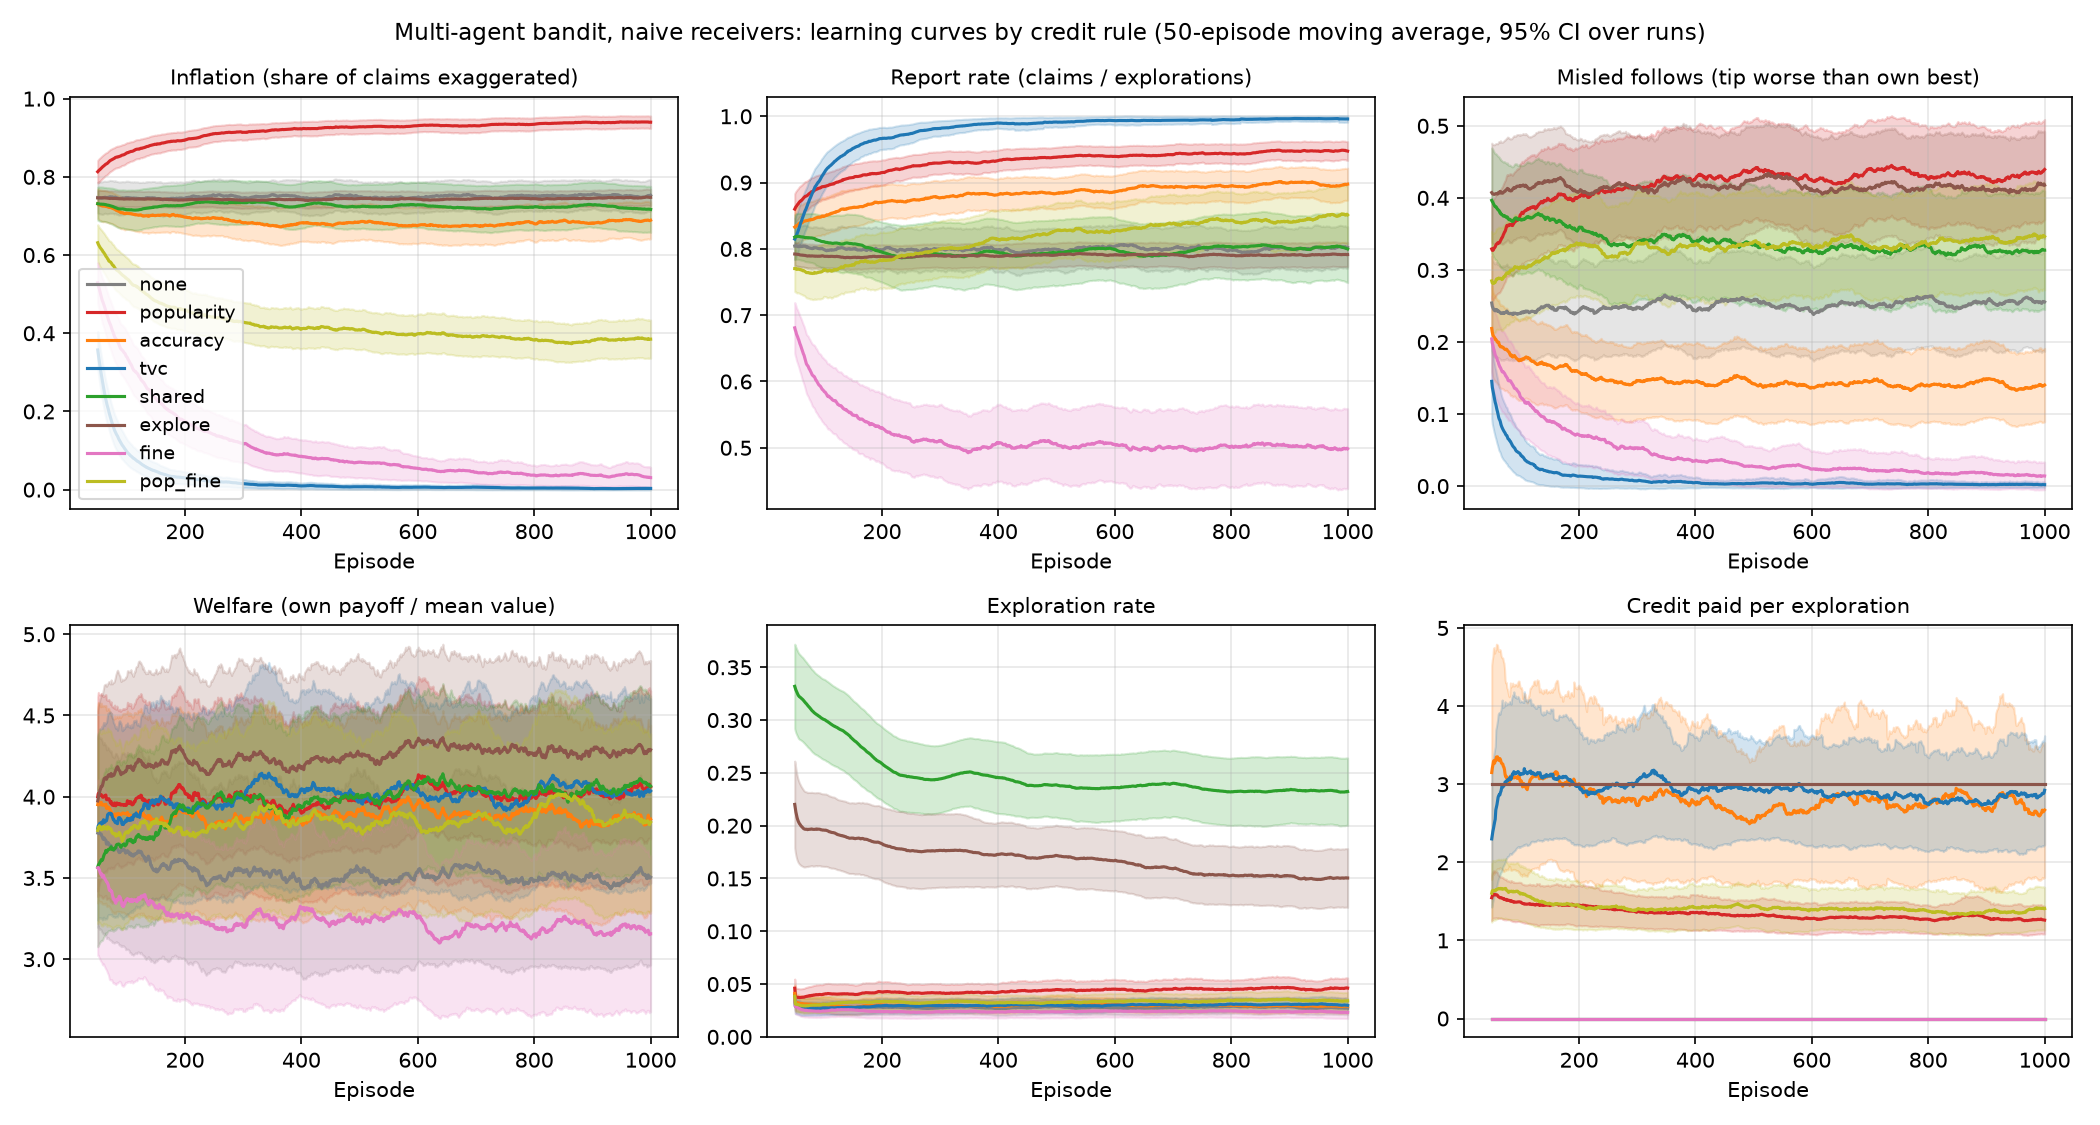
\includegraphics[width=\textwidth]{figures/bandit_naive.png}
%   \caption{Learning curves in the multi-agent bandit with naive receivers (50-episode moving average, 95\% confidence interval over 32 runs). Each panel is one metric and each line one credit design. \tvc{}'s inflation and misled follows settle near zero within about 300 episodes, popularity credit settles at high inflation, and welfare intervals overlap for most designs.}
%   \label{fig:curves-naive}
% \end{figure*}

% \begin{figure*}[t]
%   \centering
%   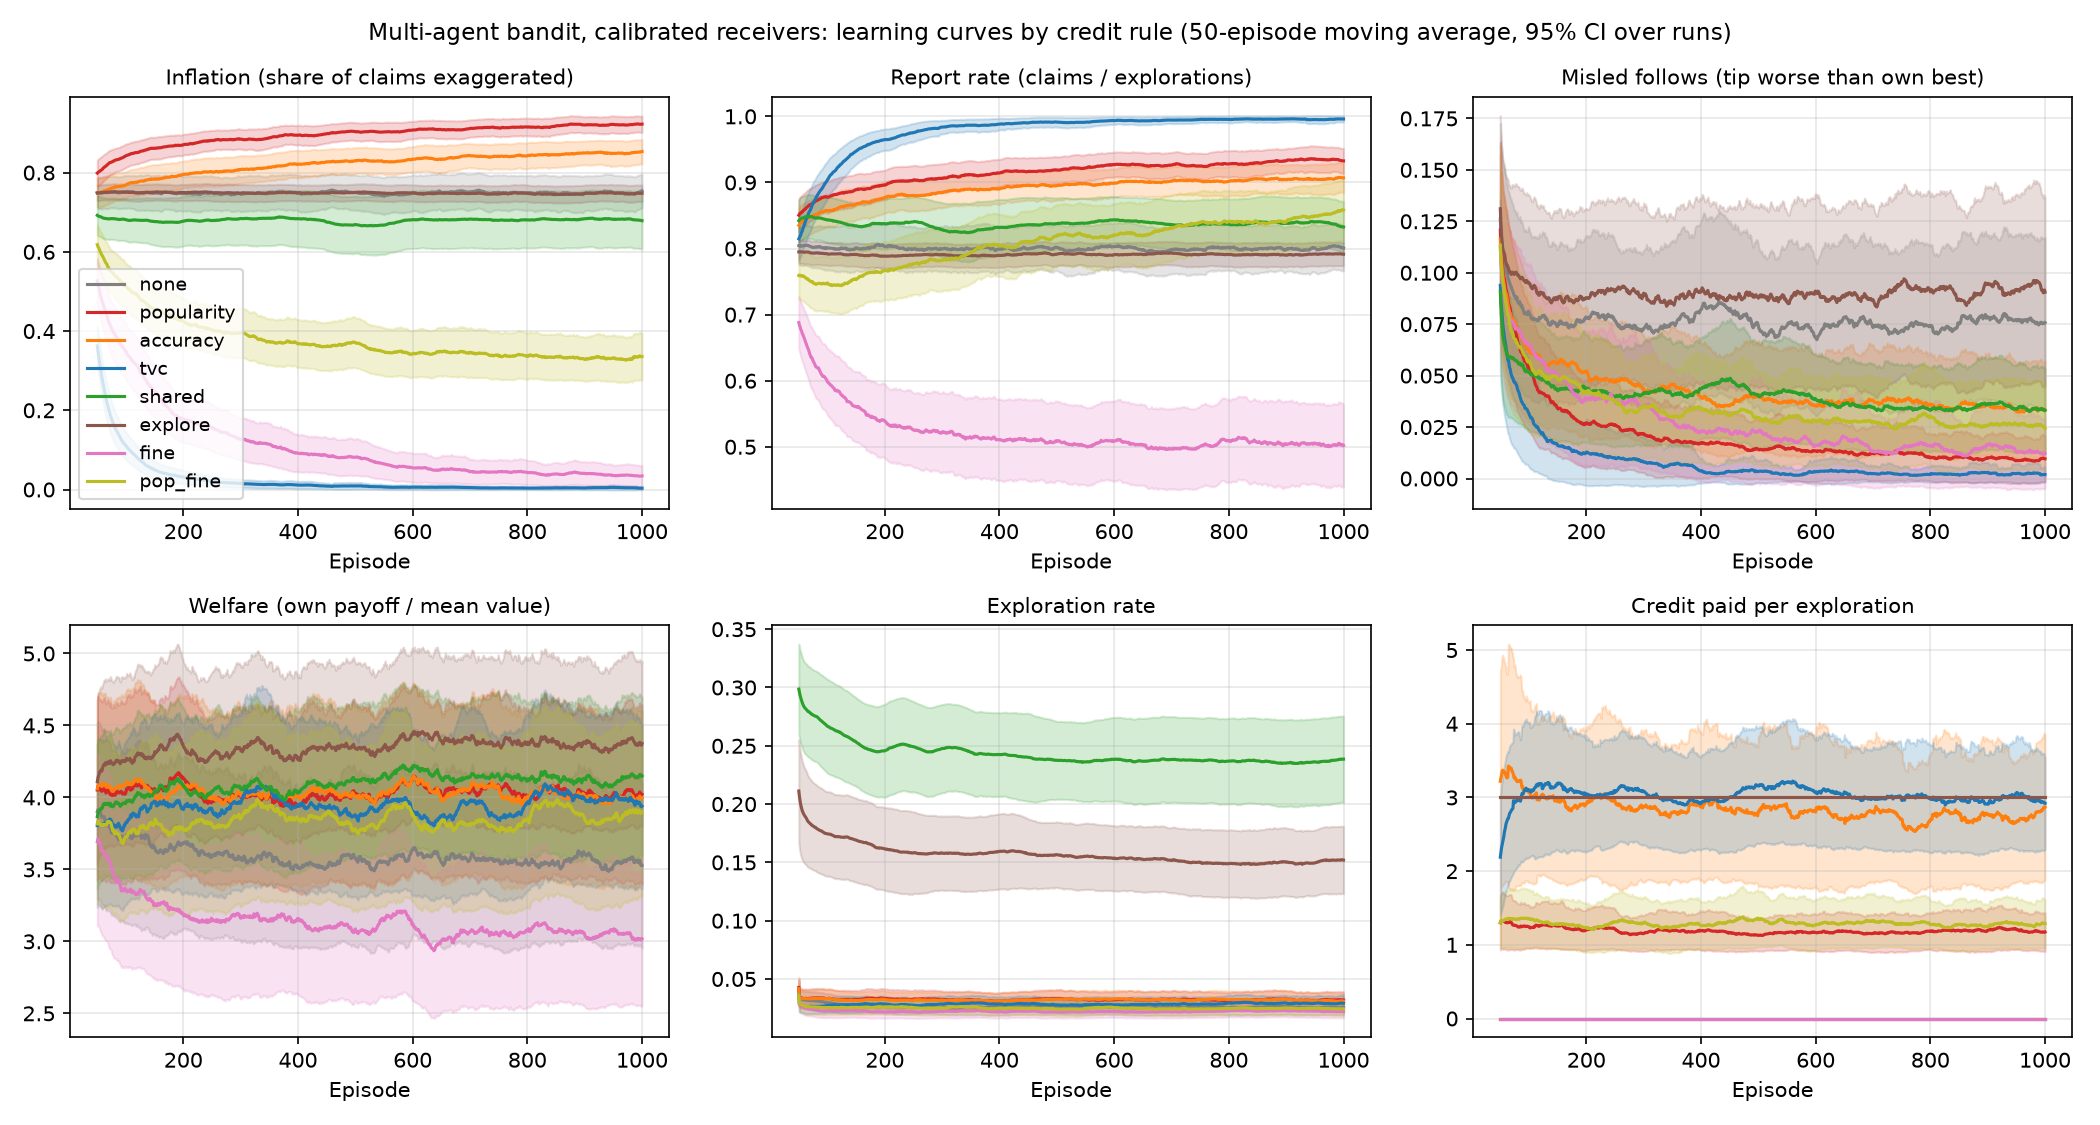
\includegraphics[width=\textwidth]{figures/bandit_calibrated.png}
%   \caption{Learning curves in the multi-agent bandit with calibrated receivers, with the same axes as \cref{fig:curves-naive}. Inflation under popularity and accuracy credit still rises slowly late in training, and under popularity credit plus a fine it still falls slowly, so the final-window means for these designs are not exact steady states.}
%   \label{fig:curves-calibrated}
% \end{figure*}

\section{Ablation Studies}
\label{app:ablation}

% \subsection{Does Lying Harm the Group?}
% To check this, we fix the claim policies instead of learning them. The first $k$ of the 12 robots post a fake jam whenever a doorway on their own route is free, the others report real jams, and no credit is given. We run 10 batches of 20 episodes for each $k$, with 95\% confidence intervals over batches. With naive receivers, group deliveries per robot per episode fall from 5.8 with no liars to 1.9 with 12 (\cref{fig:hype}), and the share of detours that were for fake jams rises from 0.31 at $k=1$ to 0.95 at $k=12$. One liar gains 3.5 deliveries over its honest peers while the others lose 0.5, so a single lie mostly moves deliveries from the others to the liar, and the group loses clearly once several robots lie. Sceptical receivers, which learn a trust for each sender from the checks they see, soften this: the group falls to 3.7 at $k=12$, and a liar's advantage at $k=1$ falls from 3.5 to 1.6. A lying robot still delivers more than an honest one at every $k<12$. Each episode starts with full trust, so this understates what trust learned over many episodes would do.

% \begin{figure*}[t]
%   \centering
%   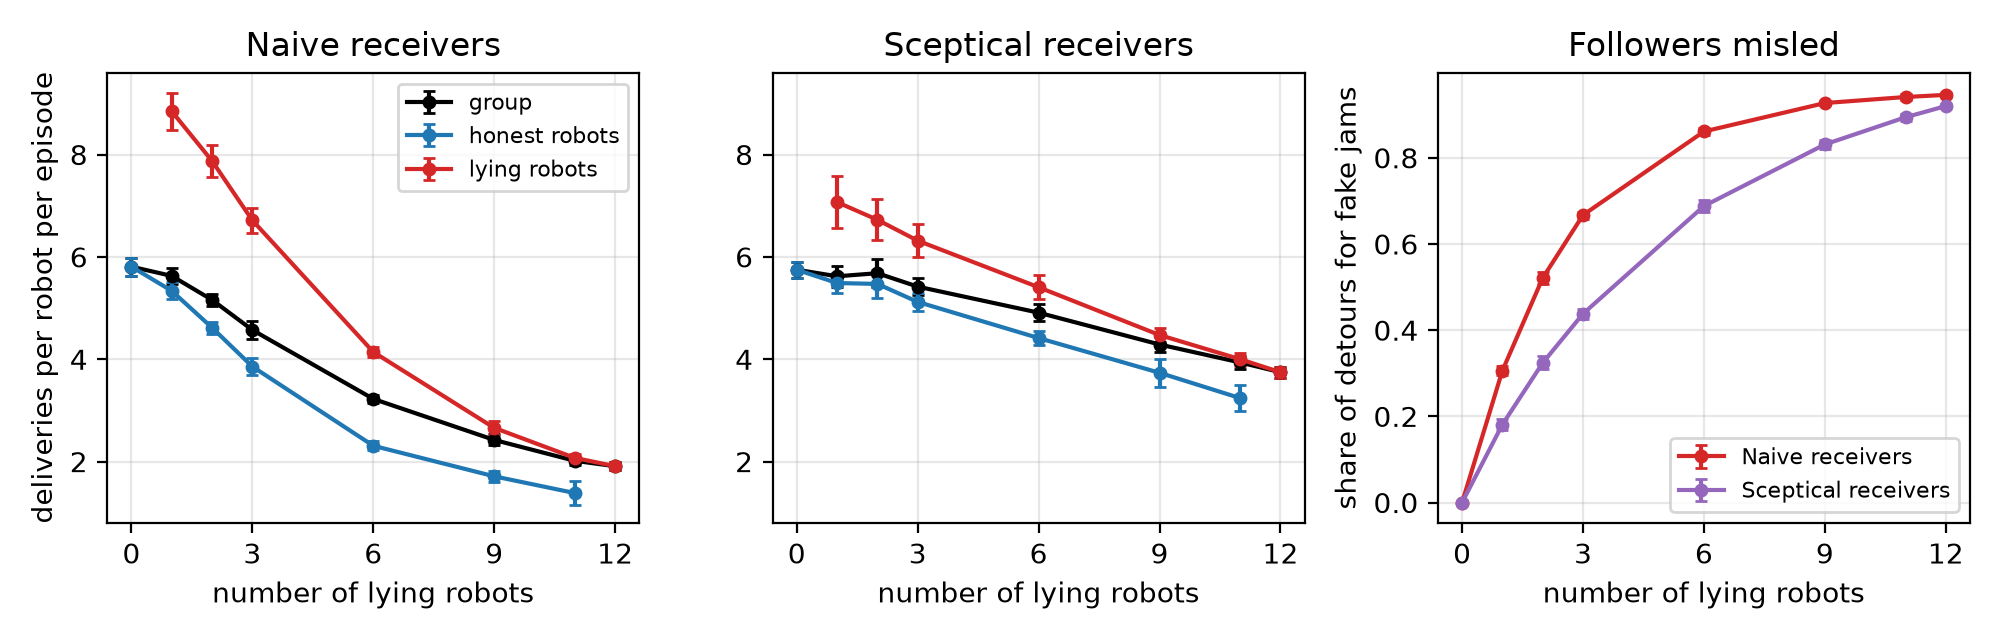
\includegraphics[width=\textwidth]{figures/fake_jams_hype_compare.png}
%   \caption{Lying harms the group in the congestion setting. The first $k$ of 12 robots post fake jams and the rest report real jams, with fixed policies and no credit (10 batches of 20 episodes, 95\% CIs). Left and middle: deliveries per robot per episode for the group, the honest robots and the lying robots, with naive and with sceptical receivers. Right: share of detours that were for fake jams.}
%   \label{fig:hype}
% \end{figure*}

% \subsection{When Do Receivers Matter?}
% To vary how much honest information changes what others do, each receiver acts on a claim only with probability $\rho$ and otherwise ignores it, with $\rho\in\{0,0.25,0.5,0.75,1\}$ and the claim policies learned as before (10 seeds). At $\rho=0$ no one acts on a claim, so a lie has no victims and an honest report helps no one, and \tvc{} adds no throughput (0.005 deliveries per robot-step with and without it, \cref{fig:listen}). Its throughput rises with $\rho$ to 0.022 at $\rho=1$, against 0.007 with no credit. Without credit the lie rate is 93--99\% whenever receivers listen, and \tvc{} holds it at 1.2\% or less at every $\rho$. The gain is not monotone at low $\rho$: at $\rho=0.25$ \tvc{} is below no credit (0.010 against 0.014). Because $\rho$ changes both whether honest information helps and whether lies have victims, this sweep does not separate the two. We therefore claim only that, in this testbed, \tvc{} raises welfare when receivers act on claims.

% \begin{figure*}[t]
%   \centering
%   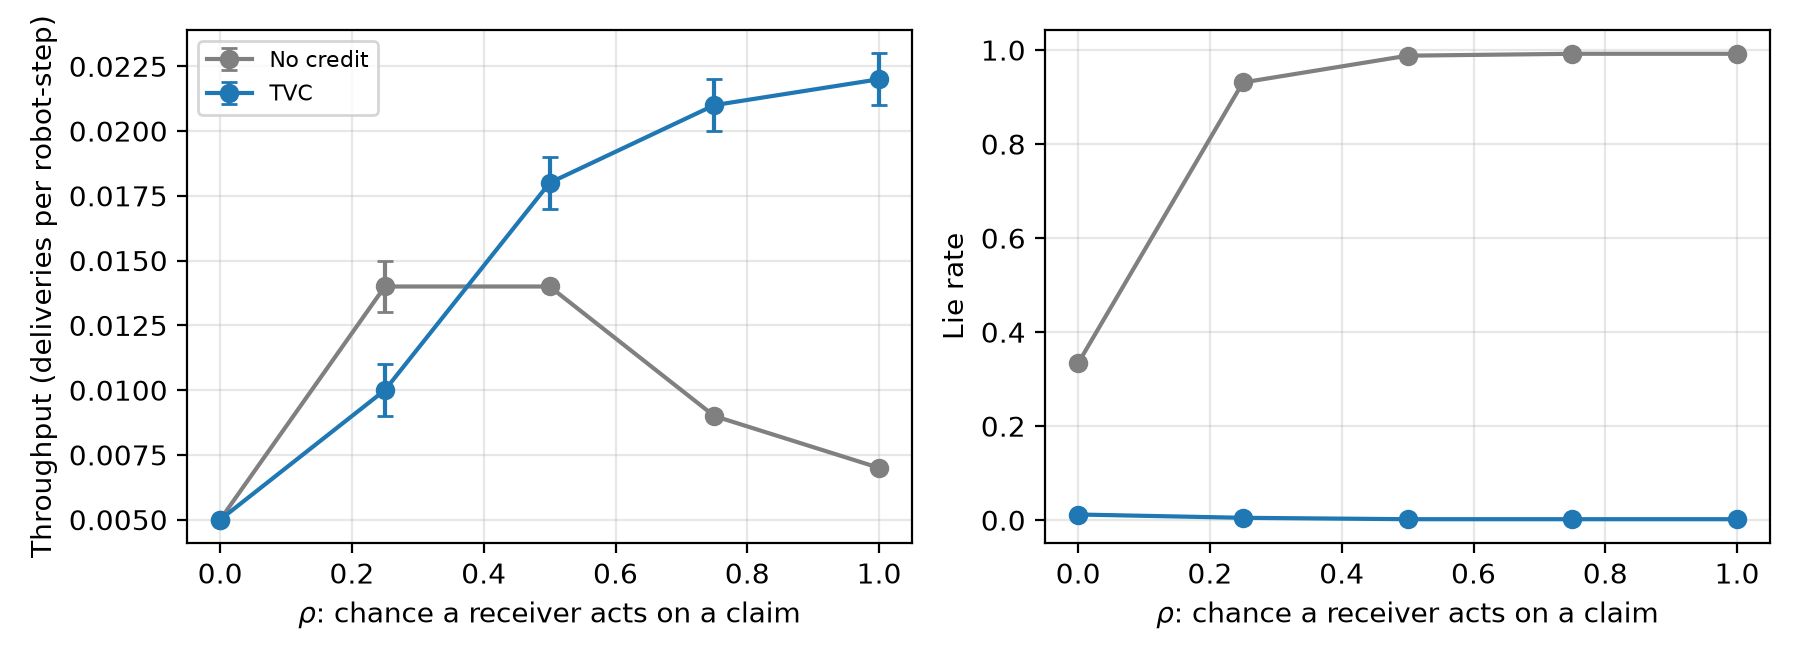
\includegraphics[width=\textwidth]{figures/fake_jams_listen.png}
%   \caption{Throughput (left) and lie rate (right) against $\rho$, the chance that a receiver acts on a claim, with no credit and with \tvc{} (10 seeds, 95\% CIs).}
%   \label{fig:listen}
% \end{figure*}

% \subsection{Which Parts of \tvc{} Are Needed?}
% We remove one part of \tvc{} at a time in the congestion setting at $\lambda=0$ (\cref{tab:ablation}; 10 seeds, 150 episodes, mean over the last 50, 95\% confidence intervals over seeds). Removing the audits ($p=0$) or the fine ($\varphi=0$) brings lying back to 99.3\% and throughput to the level of no credit. Removing the verification gate has the same effect here, because the fine is charged only on claims that fail verification, and a fake jam saves no steps, so an untruthful claim has no gain credit for the gate to block. Removing the bonus ($\eta=0$) leaves lying at 0.1\% and throughput unchanged, and lowers useful reports only slightly (96.2\% against 98.8\%), while the credit given falls from 0.040 to 0.011 per robot-step, so the bonus is not needed in this setting. Removing the cap changes nothing, because gains never reach it. This tests the parts in the congestion setting only.

% \begin{table}[t]
%   \caption{Removing one part of \tvc{} at a time in the congestion setting at $\lambda=0$ (10 seeds, mean $\pm$ 95\% CI). Lie rate and useful reports are percentages, throughput is deliveries per robot-step, and credit given is per robot-step.}
%   \label{tab:ablation}
%   \centering
%   \small
%   \setlength{\tabcolsep}{3pt}
%   \begin{tabular}{lcccc}
%     \toprule
%     Variant & Lie rate (\%) & Useful (\%) & Throughput & Credit given \\
%     \midrule
%     No credit            & $99.2 \pm 0.0$ & $44.7 \pm 1.5$ & $0.007 \pm 0.000$ & $0.000$ \\
%     Full \tvc{}          & $0.2 \pm 0.1$  & $98.8 \pm 0.7$ & $0.022 \pm 0.001$ & $0.040 \pm 0.002$ \\
%     No bonus ($\eta=0$)  & $0.1 \pm 0.0$  & $96.2 \pm 1.3$ & $0.022 \pm 0.001$ & $0.011 \pm 0.000$ \\
%     No audit ($p=0$)     & $99.3 \pm 0.0$ & $96.7 \pm 0.9$ & $0.007 \pm 0.000$ & $0.021 \pm 0.001$ \\
%     No fine ($\varphi=0$) & $99.3 \pm 0.0$ & $96.6 \pm 0.9$ & $0.007 \pm 0.000$ & $0.021 \pm 0.001$ \\
%     No gate ($\tau$ large) & $99.3 \pm 0.0$ & $96.6 \pm 0.9$ & $0.007 \pm 0.000$ & $0.021 \pm 0.001$ \\
%     No cap ($\Bbar$ large) & $0.2 \pm 0.1$  & $98.8 \pm 0.7$ & $0.022 \pm 0.001$ & $0.040 \pm 0.002$ \\
%     \bottomrule
%   \end{tabular}
% \end{table}
